\section{Introducing Non-Linearity: Activation Functions}
	
Neural networks model complex, non-linear relationships. Without non-linearity, they collapse to simple linear transformations.

\begin{abstractbox}
\textbf{Why Non-Linearity Matters:} A two-layer network without activation functions:
\begin{equation}
\vect{y} = \matr{W}_2(\matr{W}_1\vect{x} + \vect{b}_1) + \vect{b}_2 = \underbrace{\matr{W}_2\matr{W}_1}_{\matr{W}'}\vect{x} + \underbrace{\matr{W}_2\vect{b}_1 + \vect{b}_2}_{\vect{b}'}
\end{equation}
This is equivalent to a single linear layer $\vect{y} = \matr{W}'\vect{x} + \vect{b}'$. Without activation functions, depth is meaningless that implies that the mapping remains linear.
\end{abstractbox}

\begin{definition}[Activation Function]
An \textbf{activation function} $\sigma: \mathbb{R} \to \mathbb{R}$ is a non-linear function applied element-wise:
\begin{equation}
\vect{a}^{(\ell)} = \sigma(\vect{z}^{(\ell)}) = \sigma(\matr{W}^{(\ell)}\vect{a}^{(\ell-1)} + \vect{b}^{(\ell)})
\end{equation}
where $\vect{z}^{(\ell)}$ is the pre-activation and $\vect{a}^{(\ell)}$ the post-activation of layer $\ell$.
\end{definition}

Activation functions introduce non-linearity and control gradient flow during backpropagation.

\subsection{Key Properties of Activation Functions}

\subsubsection{Differentiability and Gradient Flow}

Backpropagation relies on the chain rule:
\begin{equation}
\frac{\partial \loss}{\partial z_i^{(\ell)}} = \frac{\partial \loss}{\partial a_i^{(\ell)}} \cdot \sigma'(z_i^{(\ell)})
\end{equation}

\begin{theorem}[Gradient Flow Through Layers]
The gradient with respect to layer $\ell$ parameters involves:
\begin{equation}
\frac{\partial \loss}{\partial \matr{W}^{(\ell)}} \propto \prod_{k=\ell+1}^{L} \matr{W}^{(k)} \text{diag}(\sigma'(\vect{z}^{(k-1)}))
\end{equation}
This product determines whether gradients vanish (product $\ll 1$) or explode (product $\gg 1$).
\end{theorem}

\subsubsection{Saturation and Vanishing Gradients}

\begin{definition}
An activation function $\sigma$ \textbf{saturates} in region $\mathcal{R}$ if $\lim_{x \in \mathcal{R}} |\sigma'(x)| \to 0$.
\end{definition}

\begin{calloutbox}{The Vanishing Gradient Problem}
When neurons saturate, $\sigma'(z) \approx 0$, causing:
\begin{equation}
\frac{\partial \loss}{\partial \vect{z}^{(\ell)}} \approx \frac{\partial \loss}{\partial \vect{z}^{(L)}} \cdot \prod_{k=\ell+1}^{L} \matr{W}^{(k)} \underbrace{\text{diag}(\sigma'(\vect{z}^{(k-1)}))}_{\approx 0}
\end{equation}
Gradients in early layers become exponentially small, preventing learning in deep networks with saturating activations like sigmoid and tanh.
\end{calloutbox}

\subsubsection{Zero-Centeredness}

\begin{definition}
An activation function $\sigma$ is \textbf{zero-centered} if $\sigma(0) = 0$ and $\sigma(-x) = -\sigma(x)$ (odd symmetry).
\end{definition}



\subsubsection{Sparsity}

\begin{definition}
The \textbf{sparsity} of $\sigma$ on distribution $P_X$ is:
$\text{Sparsity}(\sigma) = \Pr_{X \sim P_X}[\sigma(X) = 0]$
\end{definition}

Sparse representations offer computational efficiency, memory compression, and interpretability.

\subsection{Common Activation Functions}

Activation functions introduce non-linearities into neural networks, allowing them to learn complex patterns. They are generally categorized into classical saturating functions and modern non-saturating rectified units.

\subsubsection{Classical Functions: Sigmoid and Tanh}

Historically used in early multilayer perceptrons, these functions are now primarily used in output layers (binary classification) or specific RNN gates.

\begin{itemize}
    \item \textbf{Sigmoid:} $\sigma(x) = \frac{1}{1 + e^{-x}}$. It maps input to $(0, 1)$, allowing a probabilistic interpretation. However, it suffers from vanishing gradients (max derivative is 0.25) and outputs are not zero-centered.
    \item \textbf{Tanh:} $\tanh(x) = \frac{e^{2x} - 1}{e^{2x} + 1}$. It maps input to $(-1, 1)$. While it is zero-centered (aiding convergence), it still suffers from saturation and vanishing gradients for large $|x|$.
\end{itemize}

\begin{figure}[h]
    \centering
    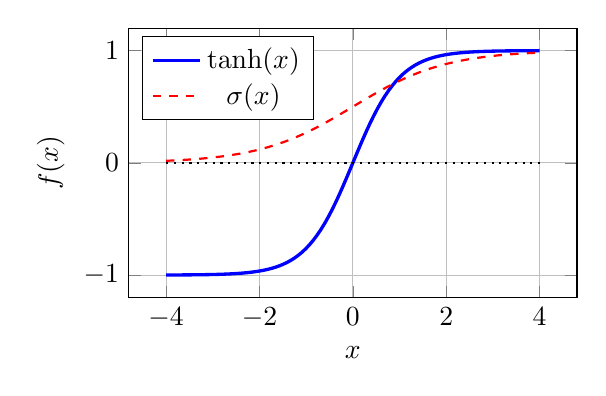
\begin{tikzpicture}
        \begin{axis}[
            width=0.6\textwidth,
            height=5cm,
            xlabel={$x$},
            ylabel={$f(x)$},
            domain=-4:4,
            samples=100,
            grid=major,
            legend pos=north west,
            ]
            \addplot[blue, very thick] {tanh(x)};
            \addplot[red, thick, dashed] {1/(1+exp(-x))};
            \addplot[black, dotted, thick] coordinates {(-4,0) (4,0)};
            \legend{$\tanh(x)$, $\sigma(x)$}
        \end{axis}
    \end{tikzpicture}
    \caption{Comparison of Tanh and Sigmoid. Tanh is zero-centered with stronger gradients near zero.}
    \label{fig:sigmoid_tanh}
\end{figure}

\subsubsection{Rectified Linear Units (ReLU) and Variants}

\paragraph{ReLU} defined as $f(x) = \max(0, x)$, became the standard for deep learning due to computational efficiency and the mitigation of the vanishing gradient problem for positive inputs. Its main drawback is the "Dying ReLU" problem, where neurons effectively die if weights update such that $wx+b < 0$ consistently.

To address this, several variants exist:
\begin{itemize}
    \item \textbf{Leaky ReLU:} $f(x) = \max(\alpha x, x)$ with a small constant $\alpha$ (e.g., 0.01) to allow gradient flow for $x < 0$.
    \item \textbf{ELU (Exponential Linear Unit):} Uses $\alpha(e^x - 1)$ for $x \le 0$. It offers smooth negative saturation and closer-to-zero mean activations but is computationally more expensive.
\end{itemize}

\subsubsection{Modern State-of-the-Art: GELU and Swish}

Recent transformer architectures (e.g., BERT, GPT) utilize smooth, non-monotonic activation functions.

\begin{itemize}
    \item \textbf{GELU (Gaussian Error Linear Unit):} $x \cdot \Phi(x)$, where $\Phi$ is the standard normal CDF. It weighs inputs by their probability, preserving information more effectively than ReLU's hard threshold.
    \item \textbf{Swish/SiLU:} $f(x) = x \cdot \sigma(\beta x)$. It is self-gated, unbounded above, and bounded below, often outperforming ReLU in deeper networks.
\end{itemize}

\begin{figure}[h]
    \centering
    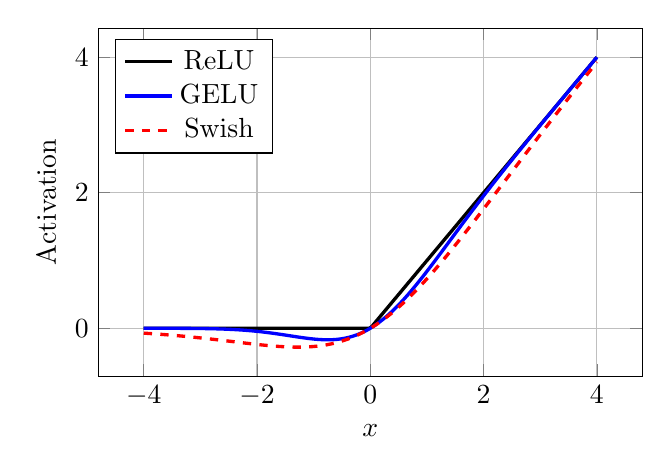
\begin{tikzpicture}
        \begin{axis}[
            width=0.7\textwidth,
            height=6cm,
            xlabel={$x$},
            ylabel={Activation},
            domain=-4:4,
            samples=200,
            grid=major,
            legend pos=north west,
            ]
            \addplot[black, very thick] {max(0,x)};
            \addplot[blue, very thick] {x * (0.5 * (1 + tanh(sqrt(2/pi) * (x + 0.044715*x^3))))};
            \addplot[red, very thick, dashed] {x/(1+exp(-x))};
            \legend{ReLU, GELU, Swish}
        \end{axis}
    \end{tikzpicture}
    \caption{Modern activation functions compared to ReLU. GELU and Swish introduce smoothness and non-monotonicity.}
    \label{fig:modern_activations}
\end{figure}

\begin{table}[h]
    \centering
    \small
    \caption{Comparison of activation function properties.}
    \begin{tabular}{@{}lcccccc@{}}
        \toprule
        \textbf{Activation} & \textbf{Range} & \textbf{Monotonic} & \textbf{Saturating} & \textbf{Zero-Centered} & \textbf{Sparse} & \textbf{Smooth} \\
        \midrule
        Sigmoid & $(0,1)$ & Yes & Both & No & No & Yes \\
        Tanh & $(-1,1)$ & Yes & Both & Yes & No & Yes \\
        ReLU & $[0,\infty)$ & Yes & Left & No & Yes & No \\
        Leaky ReLU & $(-\infty,\infty)$ & Yes & No & No & No & No \\
        ELU & $[-\alpha,\infty)$ & Yes & Left & $\approx$ Yes & No & $\approx$ Yes \\
        GELU & $(-\infty,\infty)$ & No & No & Yes & No & Yes \\
        Swish & $[-0.28,\infty)$ & No & Left & $\approx$ Yes & No & Yes \\
        \bottomrule
    \end{tabular}
\end{table}